\documentclass[11pt, spanish]{article}
\usepackage[spanish]{babel}
\selectlanguage{spanish}
\usepackage[utf8]{inputenc}
\usepackage{amsmath}
\usepackage{amsfonts}
\usepackage{amsthm}
\usepackage{float}
\usepackage{graphicx}
\pdfminorversion=5 
\pdfcompresslevel=9
\pdfobjcompresslevel=2

% Margenes
\usepackage[left=2cm,right=2cm,top=2cm,bottom=2cm]{geometry}
%Espaciado
%\linespread{1.3}


\title{Introducción al Procesamiento Digital de Imágenes - Práctica 4 (bis)}
\date{}
\author{Gonzalo Ciruelos Rodríguez (LU: 63/14)}

\begin{document}
\maketitle

Para preparar el entorno para poder ejecutar todos los programas,
primero debe tenerse instalado \texttt{python3} (y su \texttt{pip} correspondiente).
Luego, debe ejecutarse 
\begin{verbatim}
    virtualenv -p python3 venv 
    . venv/bin/activate
    pip install -r requirements.txt 
\end{verbatim}

\noindent para instalar las dependencias (pillow (para imágenes), numpy y matplotlib).



\section{Ejercicio 1.}

Transformadas de Fourier graficadas.

Modo de uso
\begin{verbatim}
    python3 practica4/ej1.py
\end{verbatim}

\subsection{Transformada de Fourier de dimensión 8 en 1D}

\[
\begin{bmatrix}
e^{\frac{-2 \pi i \cdot 0 \cdot 0}{8}} & e^{\frac{-2 \pi i \cdot 0 \cdot 1}{8}} & e^{\frac{-2 \pi i \cdot0 \cdot 2}{8}}
& e^{\frac{-2 \pi i \cdot 0 \cdot 3}{8}} & e^{\frac{-2 \pi i \cdot 0 \cdot 4}{8}} & e^{\frac{-2 \pi i \cdot 0 \cdot
5}{8}} & e^{\frac{-2 \pi i \cdot 0 \cdot 6}{8}} & e^{\frac{-2 \pi i \cdot 0 \cdot 7}{8}} \\
e^{\frac{-2 \pi i \cdot 1 \cdot 0}{8}} & e^{\frac{-2 \pi i \cdot 1 \cdot 1}{8}} & e^{\frac{-2 \pi i \cdot1 \cdot 2}{8}}
& e^{\frac{-2 \pi i \cdot 1 \cdot 3}{8}} & e^{\frac{-2 \pi i \cdot 1 \cdot 4}{8}} & e^{\frac{-2 \pi i \cdot 1 \cdot
5}{8}} & e^{\frac{-2 \pi i \cdot 1 \cdot 6}{8}} & e^{\frac{-2 \pi i \cdot 1 \cdot 7}{8}} \\
e^{\frac{-2 \pi i \cdot 2 \cdot 0}{8}} & e^{\frac{-2 \pi i \cdot 2 \cdot 1}{8}} & e^{\frac{-2 \pi i \cdot2 \cdot 2}{8}}
& e^{\frac{-2 \pi i \cdot 2 \cdot 3}{8}} & e^{\frac{-2 \pi i \cdot 2 \cdot 4}{8}} & e^{\frac{-2 \pi i \cdot 2 \cdot
5}{8}} & e^{\frac{-2 \pi i \cdot 2 \cdot 6}{8}} & e^{\frac{-2 \pi i \cdot 2 \cdot 7}{8}} \\
e^{\frac{-2 \pi i \cdot 3 \cdot 0}{8}} & e^{\frac{-2 \pi i \cdot 3 \cdot 1}{8}} & e^{\frac{-2 \pi i \cdot3 \cdot 2}{8}}
& e^{\frac{-2 \pi i \cdot 3 \cdot 3}{8}} & e^{\frac{-2 \pi i \cdot 3 \cdot 4}{8}} & e^{\frac{-2 \pi i \cdot 3 \cdot
5}{8}} & e^{\frac{-2 \pi i \cdot 3 \cdot 6}{8}} & e^{\frac{-2 \pi i \cdot 3 \cdot 7}{8}} \\
e^{\frac{-2 \pi i \cdot 4 \cdot 0}{8}} & e^{\frac{-2 \pi i \cdot 4 \cdot 1}{8}} & e^{\frac{-2 \pi i \cdot4 \cdot 2}{8}}
& e^{\frac{-2 \pi i \cdot 4 \cdot 3}{8}} & e^{\frac{-2 \pi i \cdot 4 \cdot 4}{8}} & e^{\frac{-2 \pi i \cdot 4 \cdot
5}{8}} & e^{\frac{-2 \pi i \cdot 4 \cdot 6}{8}} & e^{\frac{-2 \pi i \cdot 4 \cdot 7}{8}} \\
e^{\frac{-2 \pi i \cdot 5 \cdot 0}{8}} & e^{\frac{-2 \pi i \cdot 5 \cdot 1}{8}} & e^{\frac{-2 \pi i \cdot5 \cdot 2}{8}}
& e^{\frac{-2 \pi i \cdot 5 \cdot 3}{8}} & e^{\frac{-2 \pi i \cdot 5 \cdot 4}{8}} & e^{\frac{-2 \pi i \cdot 5 \cdot
5}{8}} & e^{\frac{-2 \pi i \cdot 5 \cdot 6}{8}} & e^{\frac{-2 \pi i \cdot 5 \cdot 7}{8}} \\
e^{\frac{-2 \pi i \cdot 6 \cdot 0}{8}} & e^{\frac{-2 \pi i \cdot 6 \cdot 1}{8}} & e^{\frac{-2 \pi i \cdot6 \cdot 2}{8}}
& e^{\frac{-2 \pi i \cdot 6 \cdot 3}{8}} & e^{\frac{-2 \pi i \cdot 6 \cdot 4}{8}} & e^{\frac{-2 \pi i \cdot 6 \cdot
5}{8}} & e^{\frac{-2 \pi i \cdot 6 \cdot 6}{8}} & e^{\frac{-2 \pi i \cdot 6 \cdot 7}{8}} \\
e^{\frac{-2 \pi i \cdot 7 \cdot 0}{8}} & e^{\frac{-2 \pi i \cdot 7 \cdot 1}{8}} & e^{\frac{-2 \pi i \cdot7 \cdot 2}{8}}
& e^{\frac{-2 \pi i \cdot 7 \cdot 3}{8}} & e^{\frac{-2 \pi i \cdot 7 \cdot 4}{8}} & e^{\frac{-2 \pi i \cdot 7 \cdot
5}{8}} & e^{\frac{-2 \pi i \cdot 7 \cdot 6}{8}} & e^{\frac{-2 \pi i \cdot 7 \cdot 7}{8}} \\
\end{bmatrix}
\]
\[=
\begin{bmatrix}
1 & 1 & 1 & 1 & 1 & 1 & 1 & 1 \\
1 & e^{\frac{-1}{4} \pi i} & e^{\frac{-1}{2} \pi i} & e^{\frac{-3}{4} \pi i} & e^{-1 \pi i} & e^{\frac{-1}{4} \pi i} &
e^{\frac{-1}{2} \pi i} & e^{\frac{-3}{4} \pi i} \\
1 & e^{\frac{-1}{2} \pi i} & e^{-1 \pi i} & e^{\frac{-1}{2} \pi i} & e^{-2 \pi i} & e^{\frac{-1}{2} \pi i} & e^{-3 \pi
i} & e^{\frac{-1}{2} \pi i} \\
1 & e^{\frac{-3}{4} \pi i} & e^{\frac{-1}{2} \pi i} & e^{\frac{-1}{4} \pi i} & e^{-3 \pi i} & e^{\frac{-3}{4} \pi i} &
e^{\frac{-1}{2} \pi i} & e^{\frac{-1}{4} \pi i} \\
1 & e^{-1 \pi i} & e^{-2 \pi i} & e^{-3 \pi i} & e^{-4 \pi i} & e^{-5 \pi i} & e^{-6 \pi i} & e^{-7 \pi i} \\
1 & e^{\frac{-1}{4} \pi i} & e^{\frac{-1}{2} \pi i} & e^{\frac{-3}{4} \pi i} & e^{-5 \pi i} & e^{\frac{-1}{4} \pi i} &
e^{\frac{-1}{2} \pi i} & e^{\frac{-3}{4} \pi i} \\
1 & e^{\frac{-1}{2} \pi i} & e^{-3 \pi i} & e^{\frac{-1}{2} \pi i} & e^{-6 \pi i} & e^{\frac{-1}{2} \pi i} & e^{-9 \pi
i} & e^{\frac{-1}{2} \pi i} \\
1 & e^{\frac{-3}{4} \pi i} & e^{\frac{-1}{2} \pi i} & e^{\frac{-1}{4} \pi i} & e^{-7 \pi i} & e^{\frac{-3}{4} \pi i} &
e^{\frac{-1}{2} \pi i} & e^{\frac{-1}{4} \pi i} \\
\end{bmatrix}
\]

\begin{figure}[H]
\centering
  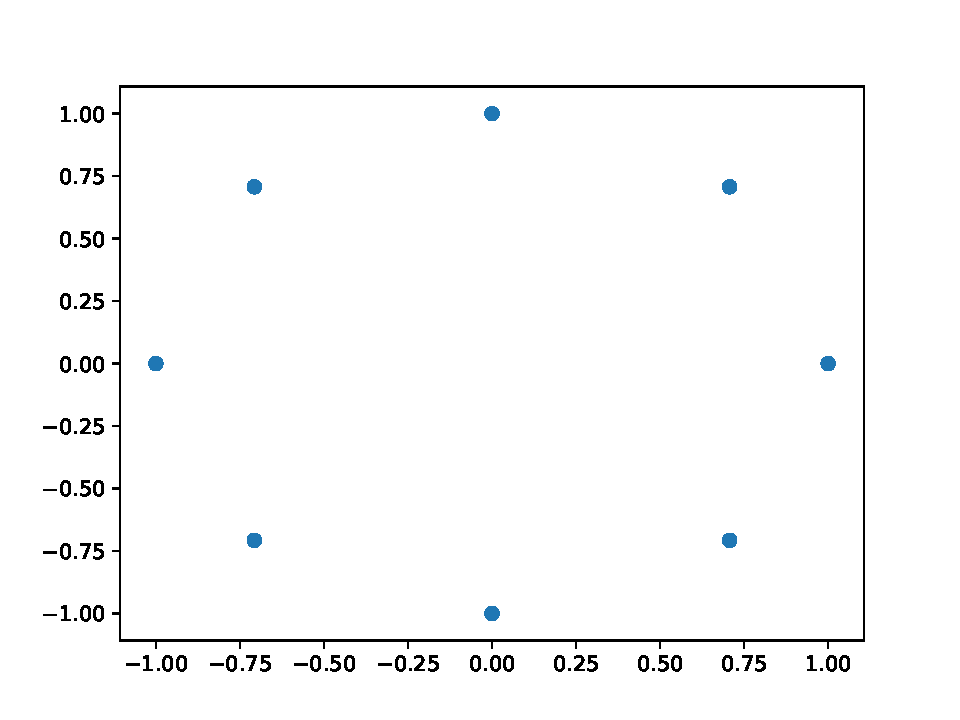
\includegraphics[height=6cm]{informe-imgs/ej1.pdf}
  \caption{\texttt{python3 practica4/ej1.py}}
\end{figure}

\subsection{Transformada de Fourier de dimensión 8 en 2D}

La matriz es de $8\times 8\times 8\times 8$, pero los puntos en el plano complejo son los mismos:

\begin{figure}[H]
\centering
  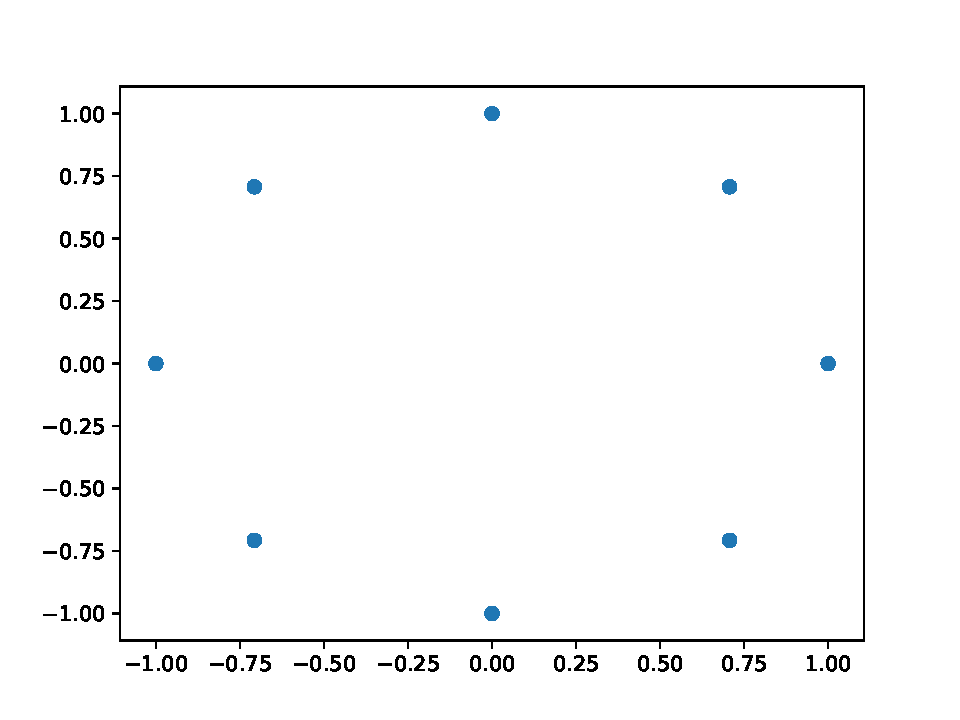
\includegraphics[height=6cm]{informe-imgs/ej1.pdf}
  \caption{\texttt{python3 practica4/ej1.py}}
\end{figure}

\newpage
\section{Ejercicio 2}
Supongamos que lo hacemos con la señal propuesta, o sea $x = [1, 1, 1, 1, 1, 1, 1, 1, 1, 0, 0, 0, 0, 0, 0, 0]$.

\begin{figure}[H]
\centering
  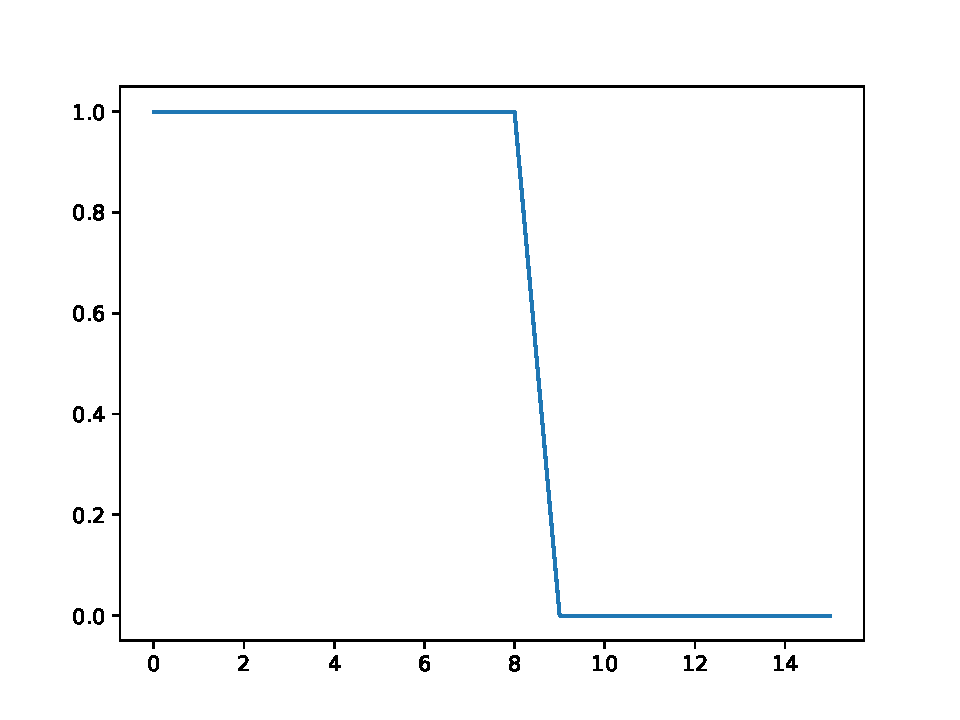
\includegraphics[height=6cm]{informe-imgs/ej2-senial.pdf}
  \caption{La señal}
\end{figure}

\subsection{Suprimiendo las frecuencias altas}

Notar que en el pasaje de la segunda señal a la tercera señal, las frecuencias más altas desaparecen.

Este es en realidad un filtro pasa bajo, con lo cual, tal como se ve, su efecto es el de suavizar un poco la señal.
\begin{figure}[H]
\centering
  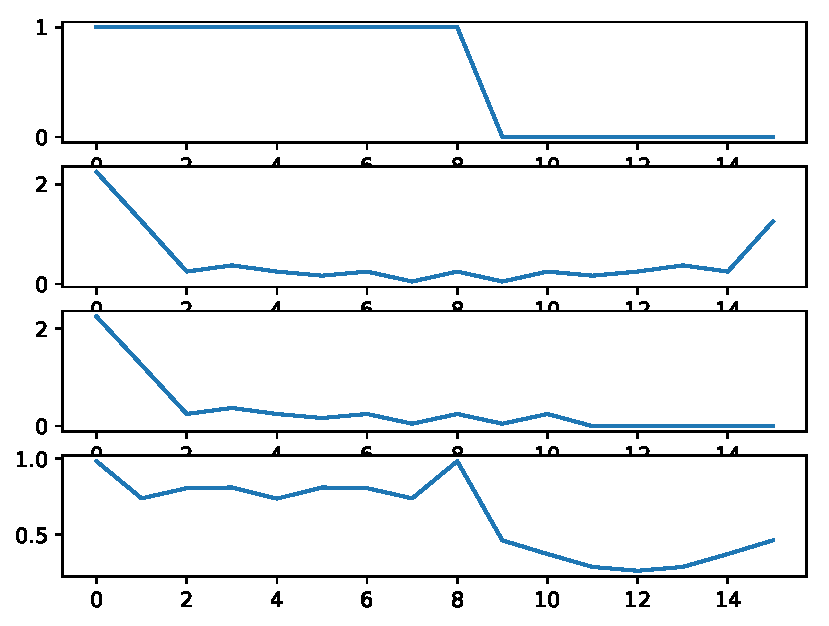
\includegraphics[height=6cm]{informe-imgs/ej2-elimino-alto.pdf}
  \caption{Filtro elimino alto. Señal original, DFT, DFT post-filtro, IDFT.}
\end{figure}

\subsection{Suprimiendo las frecuencias bajas}

Notar que en el pasaje de la segunda señal a la tercera señal, las frecuencias más bajas desaparecen.

Este es en realidad un filtro pasa alto, con lo cual el resultado es el realce de los bordes: notar que las frecuencias
más fuertes son aquellas donde la señal original tenía picos (el principio y el señal cuentan como picos pues es
periódica.

\begin{figure}[H]
\centering
  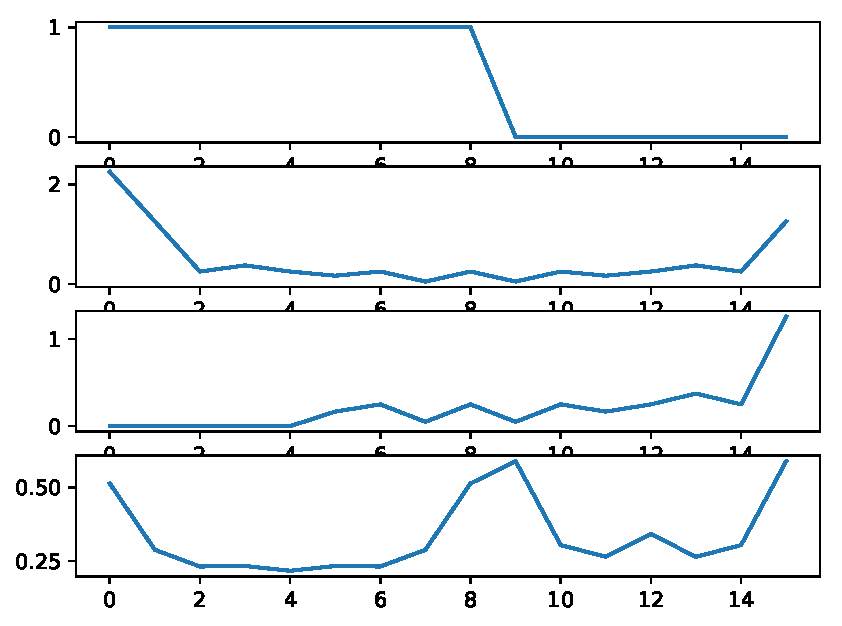
\includegraphics[height=6cm]{informe-imgs/ej2-elimino-bajo.pdf}
  \caption{Filtro elimino bajo. Señal original, DFT, DFT post-filtro, IDFT.}
\end{figure}

\subsection{Suprimiendo las frecuencias medias}

Notar que en el pasaje de la segunda señal a la tercera señal, las frecuencias del medio desaparecen.
Esto no cambia mucho la señal, pues las frecuencias intermedias ya eran bastante bajas.
\begin{figure}[H]
\centering
  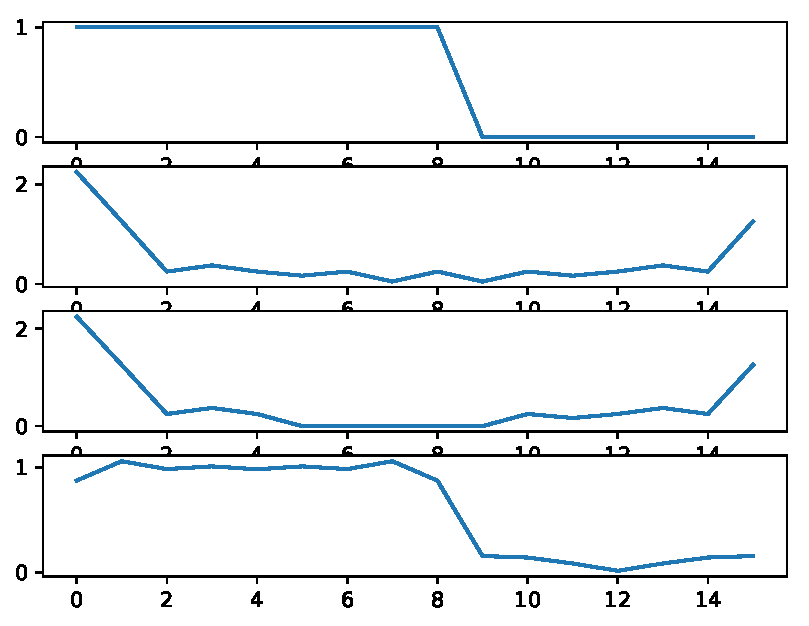
\includegraphics[height=6cm]{informe-imgs/ej2-elimino-medio.pdf}
  \caption{Filtro elimino medio. Señal original, DFT, DFT post-filtro, IDFT.}
\end{figure}

\newpage
\section{Ejercicio 6}
Fue hecho en la entrega escrita de la práctica 4.


\end{document}
